%*----------- SLIDE -------------------------------------------------------------
\begin{frame}[t]{Introdução} 
    \transdissolve[duration=0.5]
    Um dos pontos importantes na área da robótica é a interação entre os sistemas, e em decorrência ao programa de formação em robótica uma das lacunas será preenchida com o desenvolvimento do desafio 2.5..

    O desafio consiste em:
    %\newline
        \begin{columns}[t]
            \column{.05\linewidth}
            \column{.4\linewidth}
                \begin{enumerate}
                    \item assimilar o conhecimento da interação em robots;
                    \item compreender em profundidade os conceitos de simulação, e o;
                    \item desenvolvimento da liderança em projetos.
                \end{enumerate}
            \column{.6\linewidth}
            \begin{center}
            %\centerline{
                \begin{figure}
                    %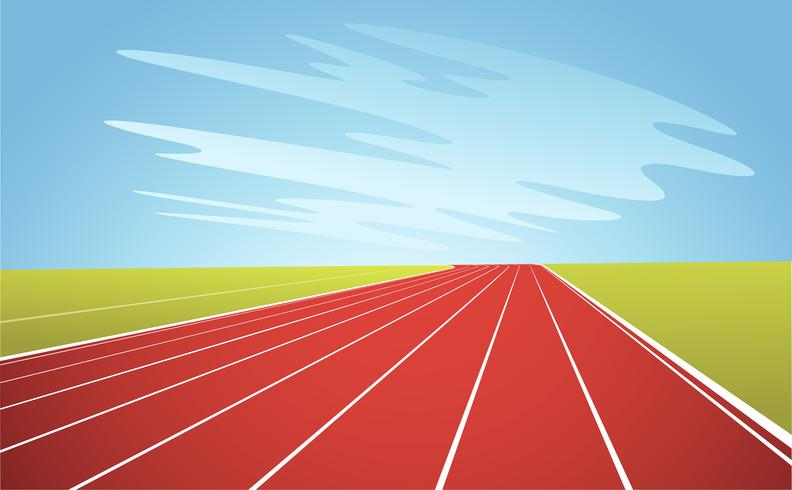
\includegraphics[width=1\textwidth]{pista}
                    \caption{Pista de corrida \cite{agostini2007}}
                    \roundpic[xshift=0cm,yshift=0cm]{4cm}{7cm}{pista}
                    %\caption{Pista de corrida \cite{agostini2007}}
                \end{figure}
            %}
            \end{center}
        \end{columns}
%*----------- notes
    \note[item]{Notes can help you to remember important information. Turn on the notes option.}
\end{frame}
%-
%*----------- SLIDE -------------------------------------------------------------
\begin{frame}[t]{O sistema robótico}
    \transboxout[duration=0.5]
    \begin{columns}
        \column{.1\textwidth}
        \column{.4\textwidth}
            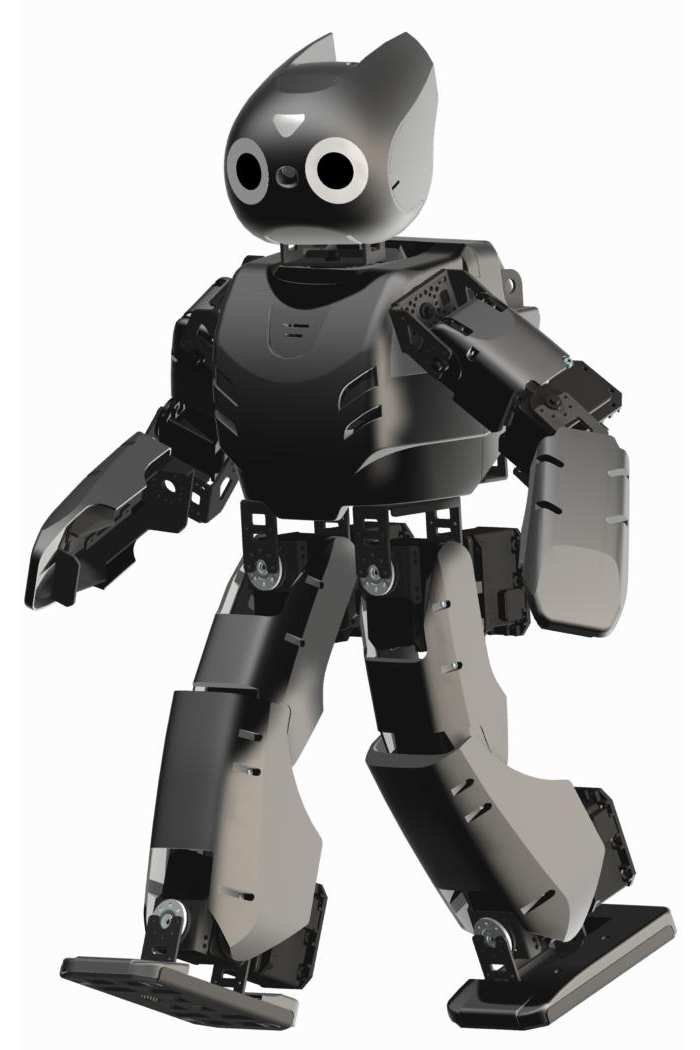
\includegraphics[width=.8\textwidth]{darwin-op}
        \column{.4\textwidth}
            \begin{enumerate}
                \item plataforma antropormórfica Darwin-OP;
                \item 20 DoF\footnote{do inglês, graus de liberdade};
                \item composto de 18 servo-motores;
                \item possui um grande gama de sensores para interação.
            \end{enumerate}
    \end{columns}
%*----------- notes
    \note[item]{Notes can help you to remember important information. Turn on the notes option.}
\end{frame}
%-
%*----------- SLIDE -------------------------------------------------------------
\begin{frame}[c]{Darwin-OP - overview}
    %\transboxin[duration=1,direction=30]
    \centering
    %   \movie[width=12.8cm,height=7.2cm,showcontrols=true,poster,autostart]
    %         {\includegraphics[width=12.8cm,height=7.2cm]{Darwin-OP}}
    %         {Darwin-OP.mp4}


          %Videos and audios don't play on Overleaf! Download the PDF and open in Acrobat Reader to view. :-)

          %This is an .mp4 file:
          
          % using a .mp4; downloaded from https://www.youtube.com/watch?v=-9iXD2-hbJM
          %\includemedia[width=0.6\linewidth,height=0.6\linewidth,activate=pageopen,passcontext,transparent,addresource=penguinschasingbutterfly.mp4,flashvars={source=penguinschasingbutterfly.mp4}]{\includegraphics[width=0.6\linewidth]{penguins}}{VPlayer.swf}
          
          %This is a YouTube video (needs an Internet connection to view):
          
          % using a YouTube video
         % \includemedia[width=0.6\linewidth,height=0.3375\linewidth,activate=pageopen,flashvars={modestbranding=1 &autohide=1 autohide &showinfo=0 &rel=0}]{\includegraphics[width=0.6\linewidth]{Darwin-OP}}{https://www.youtube.com/v/g8Ejj0T0yG4?rel=0}
          
          %This is an .mp3 file:
          %% MP3 downloaded from https://www.sample-videos.com/download-sample-audio.php
        %   \includemedia[transparent,passcontext,addresource=SampleAudio.mp3,flashvars={source=SampleAudio.mp3},]{\color{blue}\framebox[0.4\linewidth][c]{Applause}}{APlayer.swf}

    \includemedia[
      width=0.7\linewidth,
      totalheight=0.39375\linewidth,
      activate=pageopen,
      passcontext, 
      addresource=./Media/movies/Darwin-OP.mp4,
      flashvars={
      source=./Media/movies/Darwin-OP.mp4
      &autoPlay=true
      &Loop=false}
      ]{\fbox{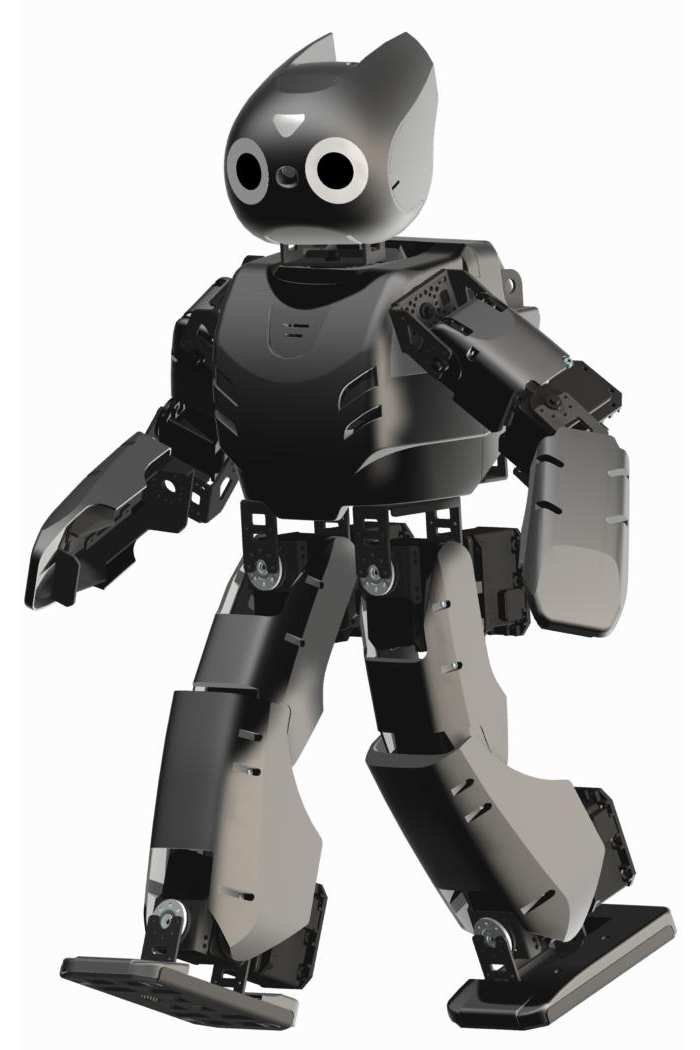
\includegraphics{darwin-op}}}{VPlayer.swf}

    %    \includemedia[
    %      width=0.4\linewidth,
    %      totalheight=0.225\linewidth,
    %      activate=pageopen,
    % %     passcontext,  %show VPlayer's right-click menu
    % %     addresource=Figures/Darwin-OP.mp4,
    %      flashvars={
    % %     %important: same path as in `addresource'
    % %     source=Figures/Darwin-OP.mp4}
    %         modestbranding=1 % no YT logo in control bar
    %         &autohide=1 % controlbar autohide
    %         &showinfo=0 % no title and other info before start
    %         &rel=0 % no related videos after end
    %         }
    %     ]{}{http://www.youtube.com/embed/1WEgNQjL66g}
    % %     &autoPlay=true
    % %     &Loop=false}
    % %     ]{\fbox{Click!}}{VPlayer.swf}

    %\pdfpcmovie{\includegraphics[width=.3\textwidth]{Darwin-OP}}{Darwin-OP.mp4}
%*----------- notes
    \note[item]{Notes can help you to remember important information. Turn on the notes option.}
\end{frame}
%-